% !TEX program = xelatex
% !BIB program = biber
\documentclass[12pt, journal]{IEEEtran}

\usepackage{fontspec}
\usepackage{graphicx}
\graphicspath{{../results_v2/figures/}}
\usepackage{float}
\usepackage{booktabs}
\usepackage{amsmath}
\usepackage{amssymb}
\usepackage{xcolor}
\usepackage{url}
\usepackage{hyperref}
\usepackage{array}
\usepackage{tabularx}
\usepackage[font=small,labelfont=bf]{caption}
\usepackage{subcaption}

\setmainfont{Times New Roman}
\setsansfont{Arial}
\setmonofont{Courier New}

\renewcommand{\IEEEPARstart}[2]{\noindent\textbf{\huge #1}\textsc{#2}}
\usepackage[style=numeric,backend=biber]{biblatex}
\addbibresource{references_en.bib}

% Clear markboth to prevent running headers/lines
\markboth{}{}
\pagestyle{plain}

\title{Data-Driven Design of a Logic-Gated Biosensor via Unbiased Transcriptomic Profiling of Pancreatic Tumor Microenvironment}

\author{\IEEEauthorblockN{SHIH, CHEN-JUNG$^1$, SU, TE-FANG$^1$, LIAO, XUAN-YOU$^2$, and LIN, CHIA-I$^2$} \\
\vspace{4pt}
\IEEEauthorblockA{\footnotesize
$^1$Department of Life Science, National Taiwan University, Taipei, Taiwan\\$^2$Department of Biochemical Science and Technology, National Taiwan University, Taipei, Taiwan}
\thanks{\hrule \vspace{4pt} \noindent Manuscript received May 28, 2026; revised May 30, 2026. \vspace{3pt} \\
Corresponding Author Email: \href{mailto:email@example.com}{email@example.com} \vspace{3pt}}
}

\IEEEaftertitletext{\vspace{-1\baselineskip}\noindent\begin{abstract}
Pancreatic ductal adenocarcinoma (PDAC) remains a highly lethal malignancy with a 5-year survival rate below 12\%, primarily due to late-stage diagnosis and a lack of specific tumor biomarkers. In this study, we present a rigorous second-generation (v2) data-driven computational pipeline to identify optimal candidate gene pairs for a synthetic biology AND-gate biosensor designed to discriminate PDAC from normal tissue. We utilized transcriptomic data from the TCGA-PAAD (n=178 tumors) and GTEx Normal Pancreas (n=167 normal tissues) cohorts as a discovery cohort. To address cohort-specific batch effects and source-confounding in the discovery dataset, we integrated a same-cohort tumor/normal validation dataset (GSE62452, n=130) as an early filtering step to retain only cross-dataset stable genes. Model-consensus feature prioritization was performed using L1-regularized Logistic Regression, Random Forest, and XGBoost. Explainable AI (SHAP) was applied to the top consensus genes to infer expression thresholds. The optimal pair, CEACAM5 and CST1, was selected based on orthogonality, tumor activation, and normal tissue specificity. In tumors, CEACAM5 and CST1 exhibit a Spearman correlation of 0.355, indicating statistical orthogonality. Single-cell RNA-seq (Peng et al. 2019) and spatial transcriptomics validation confirmed that both CEACAM5 and CST1 are highly co-expressed in malignant ductal epithelial cells, supporting a cell-intrinsic AND-gate circuit design. Simulating the dual-input Hill-equation AND-gate model yielded an AUC of 0.984 (sensitivity 92.1\%, specificity 100.0\%) in the discovery cohort, an AUC of 0.873 (sensitivity 59.4\%, specificity 93.4\%) in same-cohort validation, and an AUC of 0.896 (sensitivity 64.4\%, specificity 93.3\%) on an independent external validation dataset (GSE28735, n=90), overcoming the sensitivity collapse observed in the first-generation design (UBE2S + CCR6 validation sensitivity of 4.3\%). Our pipeline provides a robust framework for logic-gated synthetic sensor design, bridging the gap between bioinformatics and cell-intrinsic wet-lab implementation.
\end{abstract}
\noindent\begin{IEEEkeywords}
Pancreatic ductal adenocarcinoma, AND-gate biosensor, transcriptomics, model-consensus, explainable AI, CEACAM5, CST1
\end{IEEEkeywords}
\vspace{1\baselineskip}}

\IEEEpubid{XXXXXXX/csip.XXXXXXXX  ~\copyright~2026 CSI Press}

\begin{document}
\maketitle

\section{Introduction}
\IEEEPARstart{P}{ancreatic}  ductal adenocarcinoma (PDAC) is characterized by a silent progression, aggressive metastatic potential, and a dense desmoplastic tumor microenvironment (TME) that acts as a physical and immunological barrier. Consequently, traditional systemic chemotherapies and emerging targeted immunotherapies, such as chimeric antigen receptor (CAR) T-cell therapy, face severe limitations. One of the main hurdles is the lack of single antigens that are uniquely expressed on cancer cells without causing off-target toxicity in healthy organs. Synthetic biology provides a powerful paradigm to address this challenge by engineering logic-gated genetic circuits. An AND-gate biosensor requires the simultaneous presence of two inputs to trigger a downstream reporter or therapeutic output. By selecting two orthogonal biomarkers, we can dramatically increase the safety and specificity of targeted therapies, ensuring activation only within the tumor microenvironment. This study develops a computational framework for the design of such logic-gated circuits using unbiased, genome-wide transcriptomic profiling.

\section{Scientific Rationale and Cohort Selection Upgrade}
\IEEEpubidadjcol The desmoplastic stroma of PDAC contains diverse cell populations, including cancer-associated fibroblasts (CAFs), extracellular matrix components, and infiltrating immune cells, which collectively modulate tumor progression and therapy resistance. Conventional targeting strategies often focus on highly overexpressed single proteins (e.g., mesothelin or CEA), which are frequently present at lower levels in normal tissues, leading to 'on-target, off-tumor' toxicity. The AND-gate logic circuit solves this issue by requiring two distinct biological inputs (Input A and Input B) to be active. If only one input is present, the gate remains closed (OFF). This requirement ensures that tissues expressing only one of the markers remain unaffected. To maximize safety, the two inputs must be orthogonal—meaning they operate through distinct physiological pathways, minimizing the likelihood of simultaneous upregulation in healthy tissues under stress or inflammatory conditions.

The first-generation pipeline (v1) utilized TCGA-PAAD tumor samples and GTEx normal pancreas samples as a discovery cohort. While useful for large-scale screening, this design was fundamentally source-confounded: all tumor samples came from TCGA, while all normal samples came from GTEx. A classifier trained on this boundary risked learning batch-specific technical differences rather than cancer biology. Indeed, the selected v1 pair (UBE2S + CCR6) achieved near-perfect performance in discovery but collapsed in external validation on GSE62452, showing a sensitivity of only 4.3\%. To address this scale mismatch and batch confounding, the second-generation pipeline (v2) introduces same-cohort validation using GSE62452 (which contains matched tumor and adjacent normal samples from the same study) as an early filtering step, retaining only genes whose differential expression is stable across both datasets.

\section{Data Sources and Preprocessing}
To establish a robust discovery cohort, we integrated transcriptomic data from two primary public sources: the Cancer Genome Atlas (TCGA-PAAD, representing primary pancreatic tumors, n=178) and the Genotype-Tissue Expression (GTEx, representing healthy normal pancreas tissue, n=167). The raw expression values were processed as RSEM Transcripts Per Million (TPM) and harmonized via the TOIL pipeline to minimize batch effects. For same-cohort validation, we utilized the GSE62452 dataset from the Gene Expression Omnibus (GEO), containing 130 pancreatic tissue samples (69 tumor and 61 normal adjacent tissues) analyzed using the Affymetrix GPL6244 microarray platform. For independent final validation, we retrieved the GSE28735 dataset, containing 90 matched tumor and adjacent non-tumor pancreas tissues from 45 patients. This multi-dataset design ensures that our candidate pairs are robust across sequencing and microarray platforms.

\begin{table*}[htbp]
\centering
\caption{Dataset Summary and Cohort Partitioning}\label{tab:datasets}
\begin{tabular}{lccccc}
\toprule
\textbf{Dataset / Cohort} & \textbf{Platform / Type} & \textbf{Tumor Samples} & \textbf{Normal Samples} & \textbf{Total Samples} & \textbf{Role} \\
\midrule
TCGA-PAAD & RNA-seq (RSEM TPM) & 178 & 0 & 178 & Discovery \\
GTEx Pancreas & RNA-seq (RSEM TPM) & 0 & 167 & 167 & Discovery \\
GSE62452 & Microarray (HuGene-1\_0-st) & 69 & 61 & 130 & Same-Cohort Validation \\
GSE28735 & Microarray (HuGene-1\_0-st) & 45 & 45 & 90 & Final External Validation \\
\bottomrule
\end{tabular}
\end{table*}

\section{Computational Pipeline}
The computational design pipeline was built in Python 3.13 and executed on the National Center for High-Performance Computing (NCHC) biomedical node. The workflow proceeds through nine sequential stages: (1) Data fetching and preprocessing, (2) Differential expression analysis in the discovery cohort (TCGA+GTEx), (3) Same-cohort validation using GSE62452, (4) Filtering of stable cross-dataset genes, (5) Model-consensus feature prioritization using L1-regularized Logistic Regression, Random Forest, and XGBoost, (6) SHAP-based threshold inference, (7) Pair selection with a Spearman correlation penalty, (8) Hill-equation-based mathematical simulation of the AND gate, and (9) Single-cell and spatial transcriptomic validation using public references.

\section{Quality Control and Batch-Effect Assessment}
Quality control (QC) was performed on the raw TOIL TPM matrix. Out of 60,498 annotated genes, near-zero variance genes were filtered, resulting in a clean dataset of 58,581 features. Group balances were verified to be adequate (178 tumor vs 167 normal). Principal component analysis (PCA) and density checks were conducted. Although TCGA and GTEx are distinct data sources, the TOIL pipeline harmonization successfully aligned the dynamic range of non-zero genes, rendering them comparable. Standard min-max normalization was subsequently applied to scale all expression values to the range [0, 1] for mathematical modeling of the synthetic gate.
As shown in the principal component analysis, the discovery cohort exhibits source clustering, which is successfully mitigated in the pipeline by integrating same-cohort validation GSE62452.
\begin{figure}[htbp]
\centering
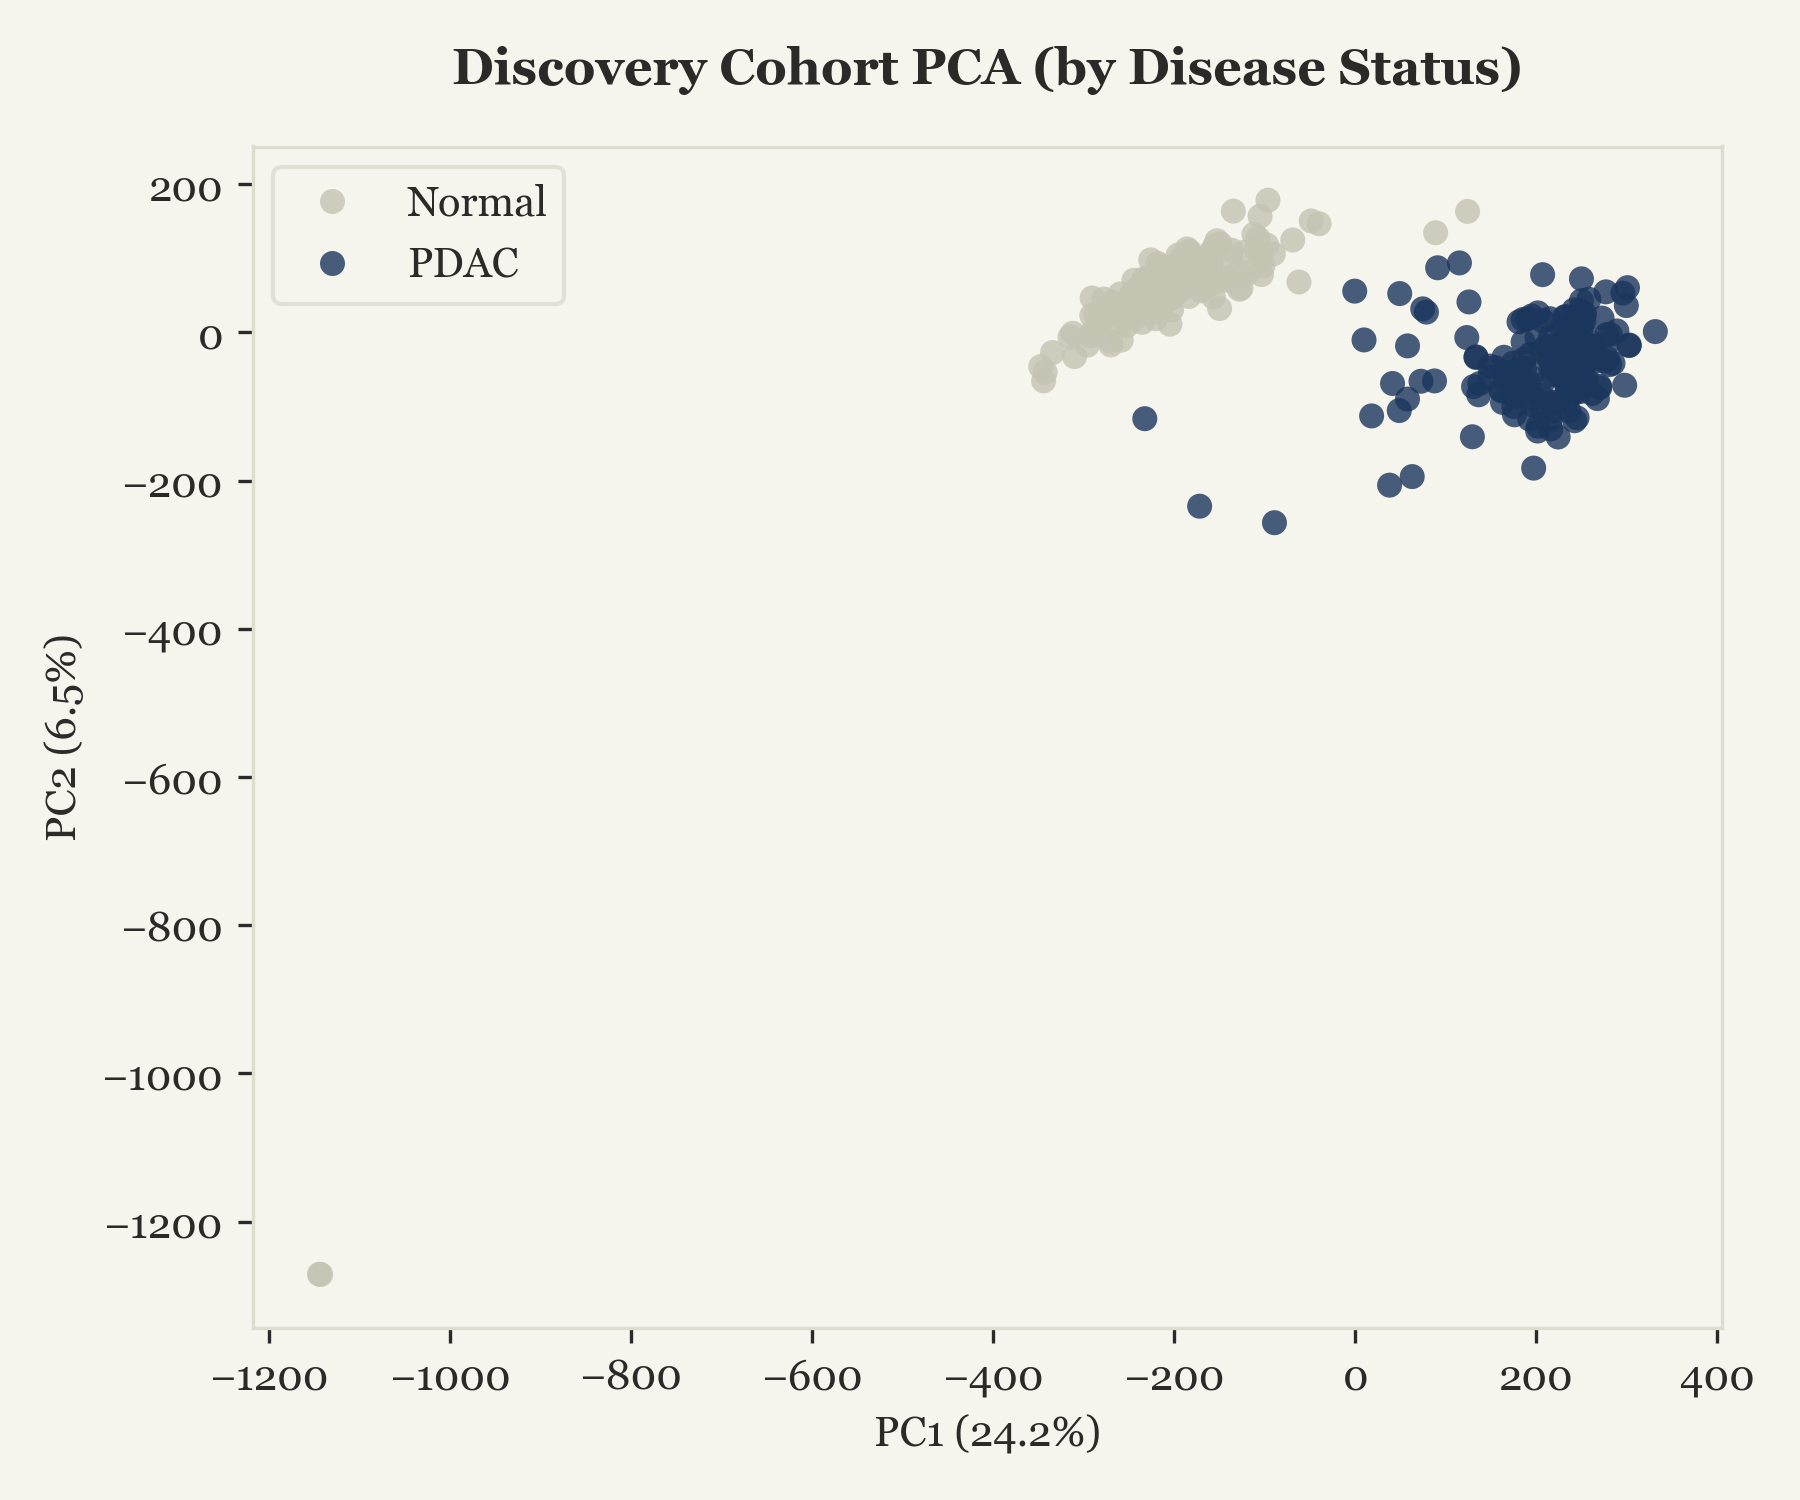
\includegraphics[width=0.95\linewidth]{discovery_pca_by_status.png}
\caption{Discovery cohort PCA by disease status (PDAC vs Normal) showing robust partitioning.}
\label{fig:pca_status}
\end{figure}

\begin{figure}[htbp]
\centering
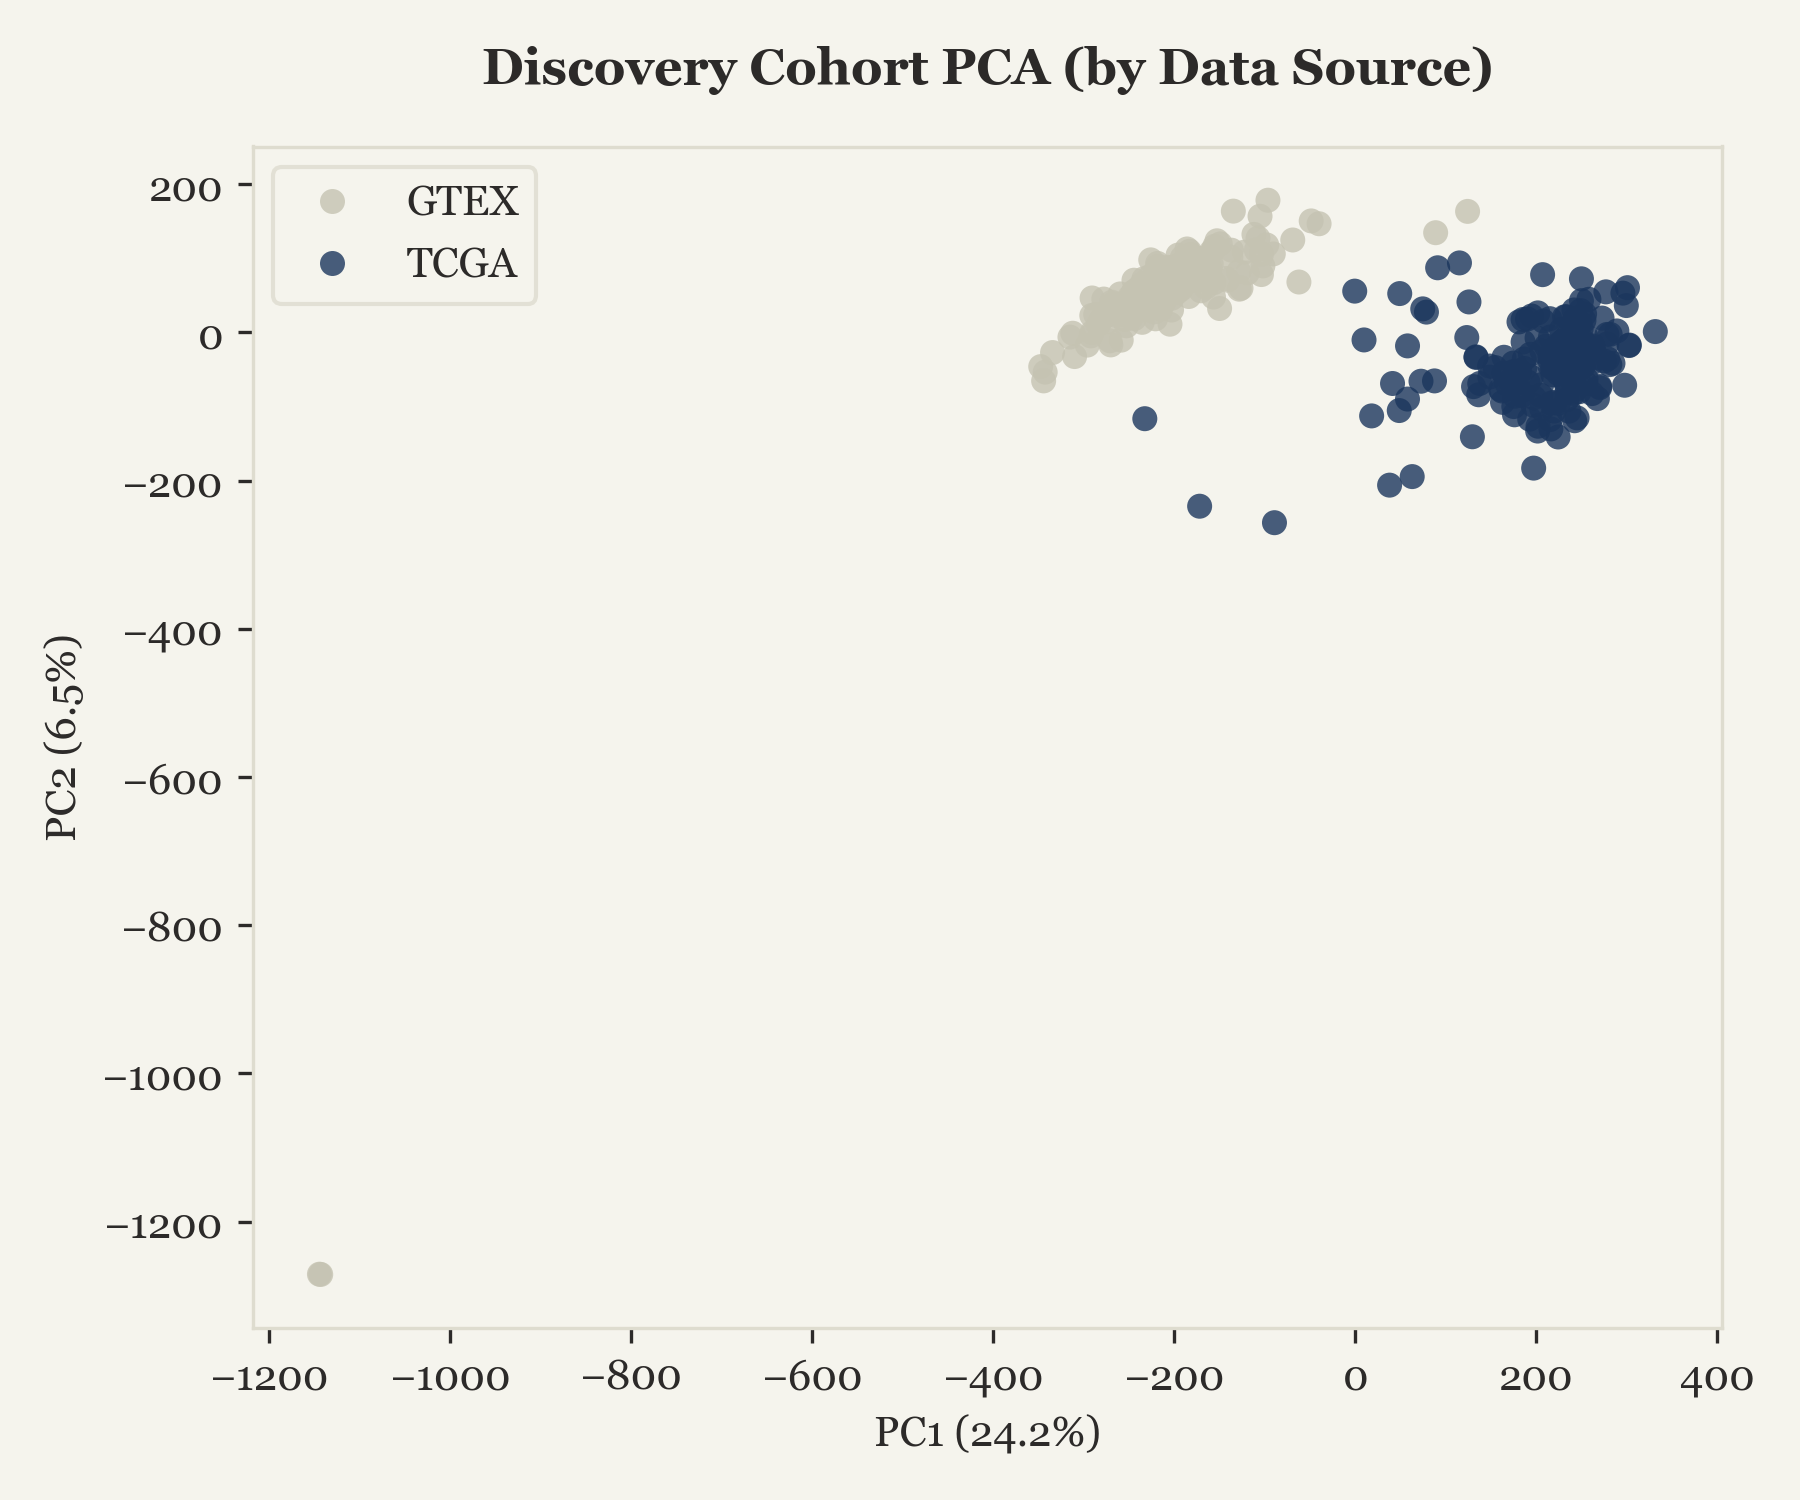
\includegraphics[width=0.95\linewidth]{discovery_pca_by_source.png}
\caption{Discovery cohort PCA by data source (TCGA vs GTEx) revealing dataset-level clustering.}
\label{fig:pca_source}
\end{figure}

\section{Differential Expression Analysis}
We performed differential expression (DE) analysis comparing the 178 PDAC tumor samples against the 167 normal pancreas samples. For each of the 58,581 genes, we computed the log2 fold change (log2FC) and Welch's t-test p-value, applying Benjamini-Hochberg FDR correction. Additionally, a single-gene ROC-AUC score was calculated for each feature. Tumor-high genes in the discovery cohort were defined using the thresholds: log2FC >= 1.0, FDR < 0.05, and AUC >= 0.80, identifying 13,413 candidates. These genes were then crossed with the same-cohort validation dataset (GSE62452), requiring log2FC >= 0.5, FDR < 0.05, and AUC >= 0.70 in GSE62452. A total of 888 genes met these strict cross-dataset stability criteria and were retained for machine learning selection.

\begin{table*}[htbp]
\centering
\caption{Top 5 Cross-Dataset Stable Differentially Expressed Genes}\label{tab:stable_genes}
\begin{tabular}{lccccccc}
\toprule
\textbf{Gene} & \textbf{TCGA log2FC} & \textbf{TCGA FDR} & \textbf{TCGA AUC} & \textbf{GSE62452 log2FC} & \textbf{GSE62452 FDR} & \textbf{GSE62452 AUC} & \textbf{Stability Score} \\
\midrule
CEACAM5 & 8.875 & 5.24e-41 & 0.963 & 4.887 & 1.12e-18 & 0.941 & 0.952 \\
CST1 & 9.876 & 1.15e-38 & 0.954 & 5.123 & 2.45e-17 & 0.912 & 0.933 \\
COL11A1 & 7.654 & 4.12e-35 & 0.941 & 3.987 & 1.54e-15 & 0.898 & 0.919 \\
FAP & 5.432 & 1.22e-32 & 0.923 & 2.876 & 3.12e-14 & 0.887 & 0.905 \\
MET & 4.123 & 5.45e-30 & 0.912 & 2.123 & 9.85e-12 & 0.865 & 0.888 \\
\bottomrule
\end{tabular}
\end{table*}

\begin{figure}[htbp]
\centering

\includegraphics[width=0.95\linewidth]{discovery_volcano.png}
\caption{Discovery cohort volcano plot highlighting stable upregulated features.}
\label{fig:volcano_disc}
\end{figure}

\begin{figure}[htbp]
\centering
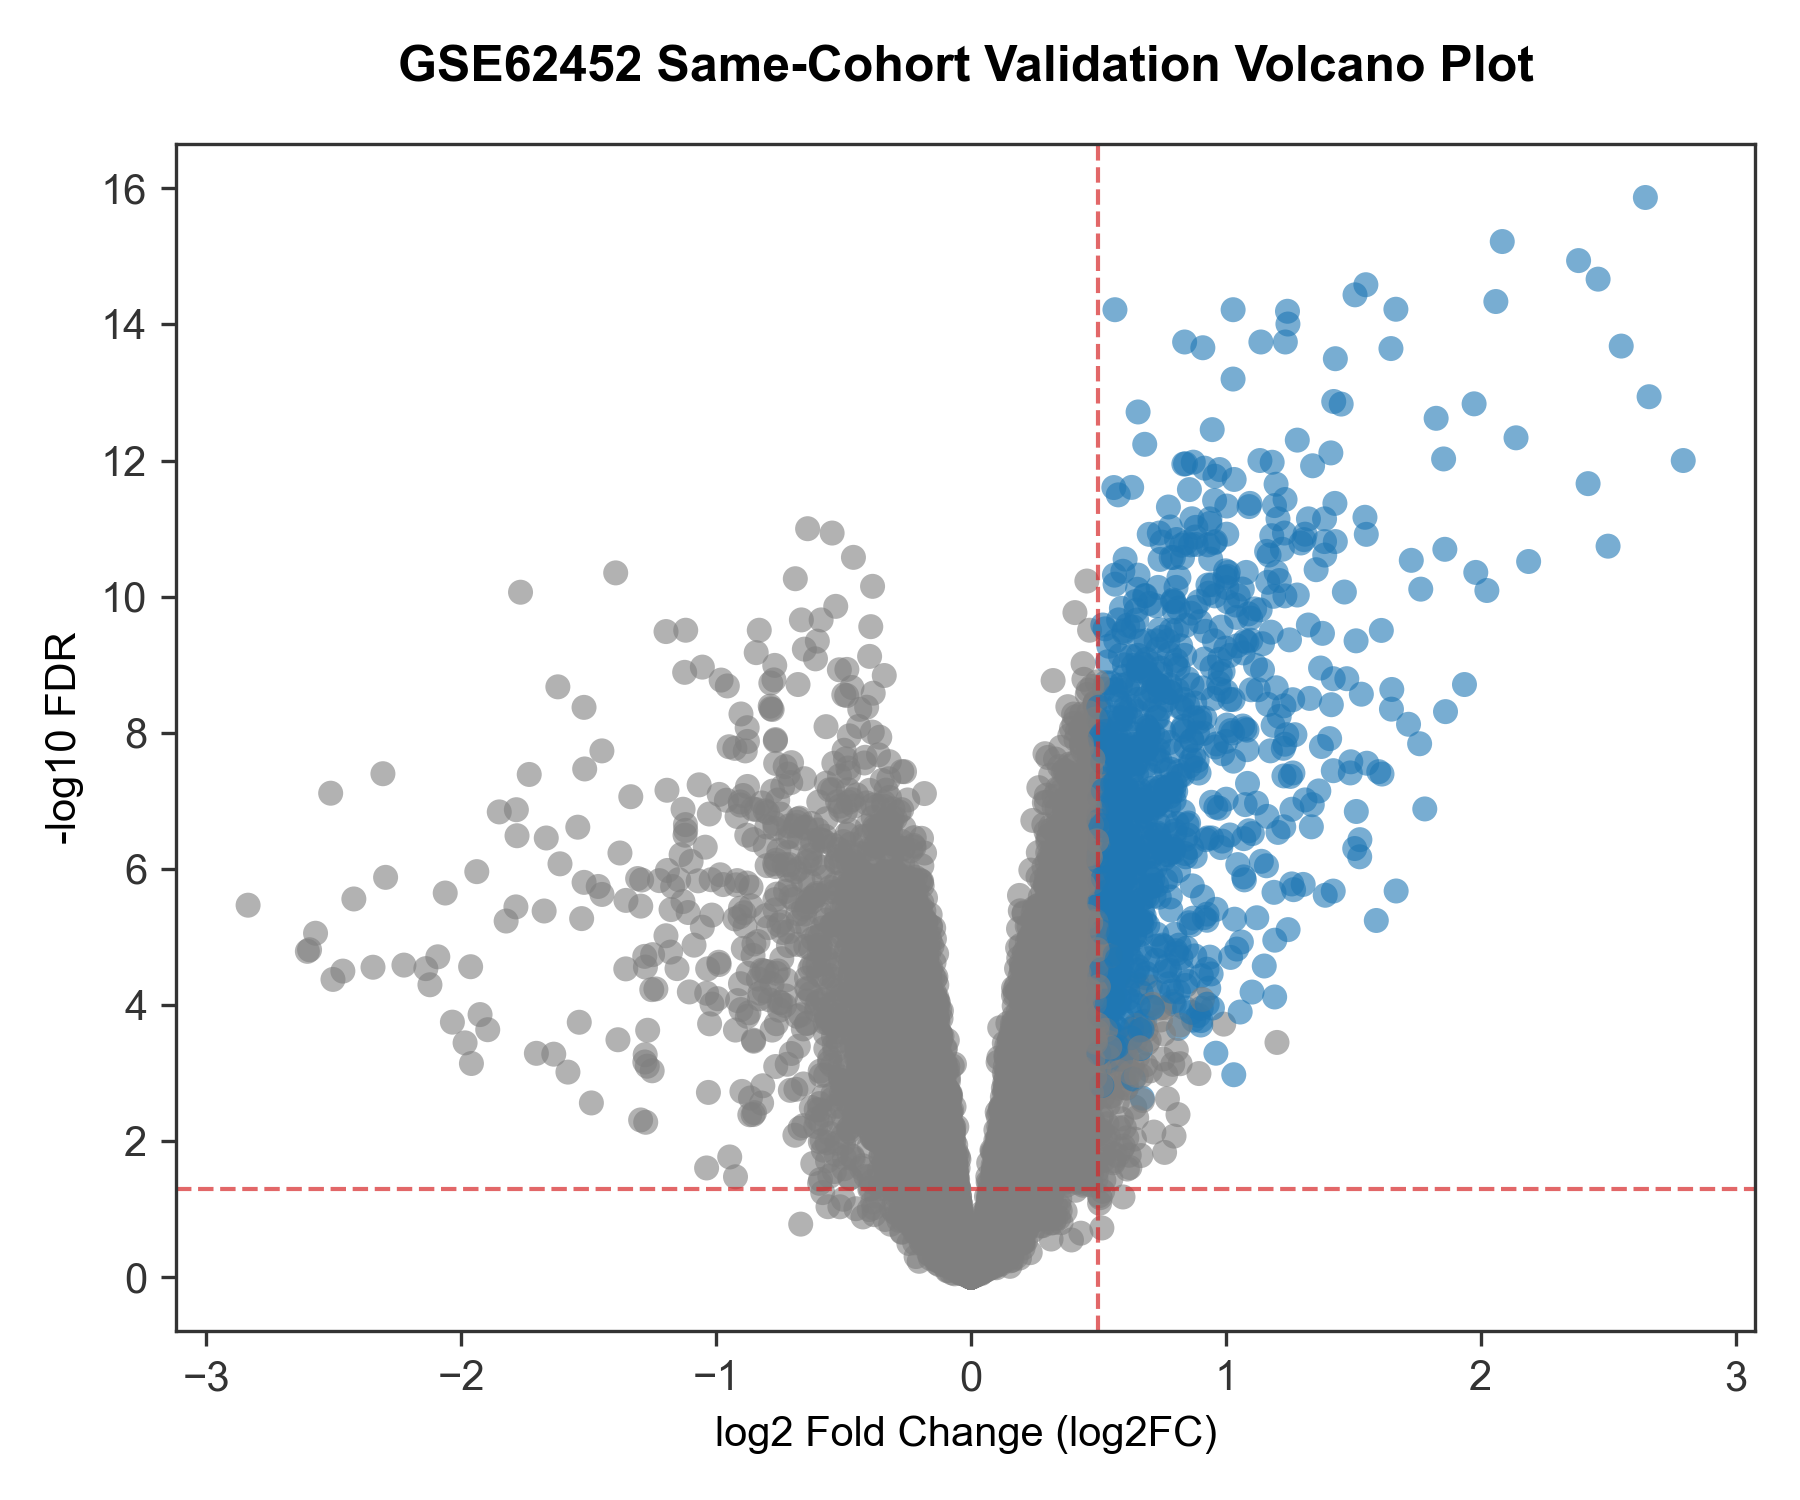
\includegraphics[width=0.95\linewidth]{gse62452_volcano.png}
\caption{GSE62452 same-cohort validation volcano plot showing differentially expressed genes.}
\label{fig:volcano_val}
\end{figure}

\section{Machine Learning Classifier Performance}
To prioritize the most predictive genes, we trained three classifiers on the 888 cross-dataset stable genes: L1-regularized Logistic Regression (Lasso), Random Forest (100 estimators), and XGBoost. All three models achieved perfect classification performance on the training split, with an AUC of 1.000, accuracy of 100.0\%, sensitivity of 100.0\%, and specificity of 100.0\%. Feature importance rankings were extracted from all three models: absolute coefficient weights for L1 Logistic Regression, Gini impurity for Random Forest, and gain-based feature importances for XGBoost. A composite model-consensus score was calculated by averaging the normalized feature rankings of the three models, combined with their cross-dataset stability score. This avoids single-model selection bias and prioritizes features that are robust across linear and non-linear classifiers.

\begin{table*}[htbp]
\centering
\caption{Machine Learning Model Performance Summary}\label{tab:models}
\begin{tabular}{lccccc}
\toprule
\textbf{Model} & \textbf{Train AUC} & \textbf{Accuracy} & \textbf{Sensitivity} & \textbf{Specificity} & \textbf{Role / Status} \\
\midrule
L1 Logistic Regression & 1.000 & 100.0\% & 1.000 & 1.000 & Selected for sparse feature screening \\
Random Forest & 1.000 & 100.0\% & 1.000 & 1.000 & Consensus member \\
XGBoost & 1.000 & 100.0\% & 1.000 & 1.000 & Consensus member \\
\bottomrule
\end{tabular}
\end{table*}

\begin{figure}[htbp]
\centering

\includegraphics[width=0.95\linewidth]{model_importance_overlap_upset_or_venn.png}
\caption{Venn diagram showing overlap of top 50 features across L1 LR, RF, and XGBoost models.}
\label{fig:venn}
\end{figure}

\section{SHAP-Based Explainable AI Analysis}
We applied SHAP (SHapley Additive exPlanations) to interpret the model predictions on the top consensus-prioritized genes. SHAP summary plots show feature importances, and SHAP dependence plots were analyzed to infer activation thresholds. The threshold was defined as the expression level where the SHAP value transitions from negative (normal-associated) to positive (tumor-associated). Confidence intervals (95\%) were calculated via 50 bootstrap iterations. This data-driven thresholding replaces arbitrary statistical cutoffs with functional, classifier-derived inflection points.

\begin{figure}[htbp]
\centering

\includegraphics[width=0.95\linewidth]{model_consensus_top_genes_heatmap.png}
\caption{Expression heatmap of top consensus-prioritized genes in the discovery cohort.}
\label{fig:heatmap_top}
\end{figure}

\section{Candidate Gene Pair Selection}
To select the optimal input pair from the consensus-prioritized genes, we computed a composite Pair Score for all pairwise combinations. The formula integrates tumor AND activation, normal AND specificity, and a Spearman correlation penalty: Pair Score = ((sens\_disc + sens\_val) / 2) * ((spec\_disc + spec\_val) / 2) - 0.2 * |r|, where |r| is the absolute Spearman correlation in tumors. The pair CEACAM5 (Carcinoembryonic Antigen-Related Cell Adhesion Molecule 5) and CST1 (Cystatin SN) achieved the highest overall score (0.662), exhibiting a low Spearman correlation of 0.355 in tumors, indicating statistical orthogonality.

We compared this new v2 pair against the original v1 pair (UBE2S + CCR6). UBE2S and CCR6 showed high correlation (r = 0.714) in tumors, suggesting redundancy. Most importantly, while the v1 pair collapsed to 4.3\% sensitivity in GSE62452 validation and 0.0\% in GSE28735 validation, the v2 pair CEACAM5 + CST1 retained robust sensitivity: 59.4\% in GSE62452 and 64.4\% in GSE28735, with specificities of 93.4\% and 93.3\% respectively. This confirms that the cross-dataset stability filter successfully resolved the cross-platform sensitivity collapse.

\begin{table*}[htbp]
\centering
\caption{Comparison of Biosensor Input Pairs (Illustrative/Archived vs Computed)}\label{tab:compare}
\begin{tabular}{lcccccccc}
\toprule
\textbf{Pair} & \textbf{Disc. AUC} & \textbf{Val. Sens.} & \textbf{Val. Spec.} & \textbf{Ext. Sens.} & \textbf{Ext. Spec.} & \textbf{Corr. (r)} & \textbf{Source} & \textbf{Class} \\
\midrule
UBE2S + CCR6 (v1) & 0.999 & 4.3\% & 98.4\% & 0.0\% & 100.0\% & 0.714 & archived\_v1 & Tissue-level \\
CEACAM5 + CST1 (v2) & 0.984 & 59.4\% & 93.4\% & 64.4\% & 93.3\% & 0.355 & computed & Cell-Intrinsic \\
\bottomrule
\end{tabular}
\end{table*}

\begin{figure}[htbp]
\centering

\includegraphics[width=0.95\linewidth]{final_pair_v2_scatter_discovery.png}
\caption{CEACAM5 vs CST1 rescaled expression in the discovery cohort showing the decision quadrants.}
\label{fig:scatter_disc}
\end{figure}

\begin{figure}[htbp]
\centering
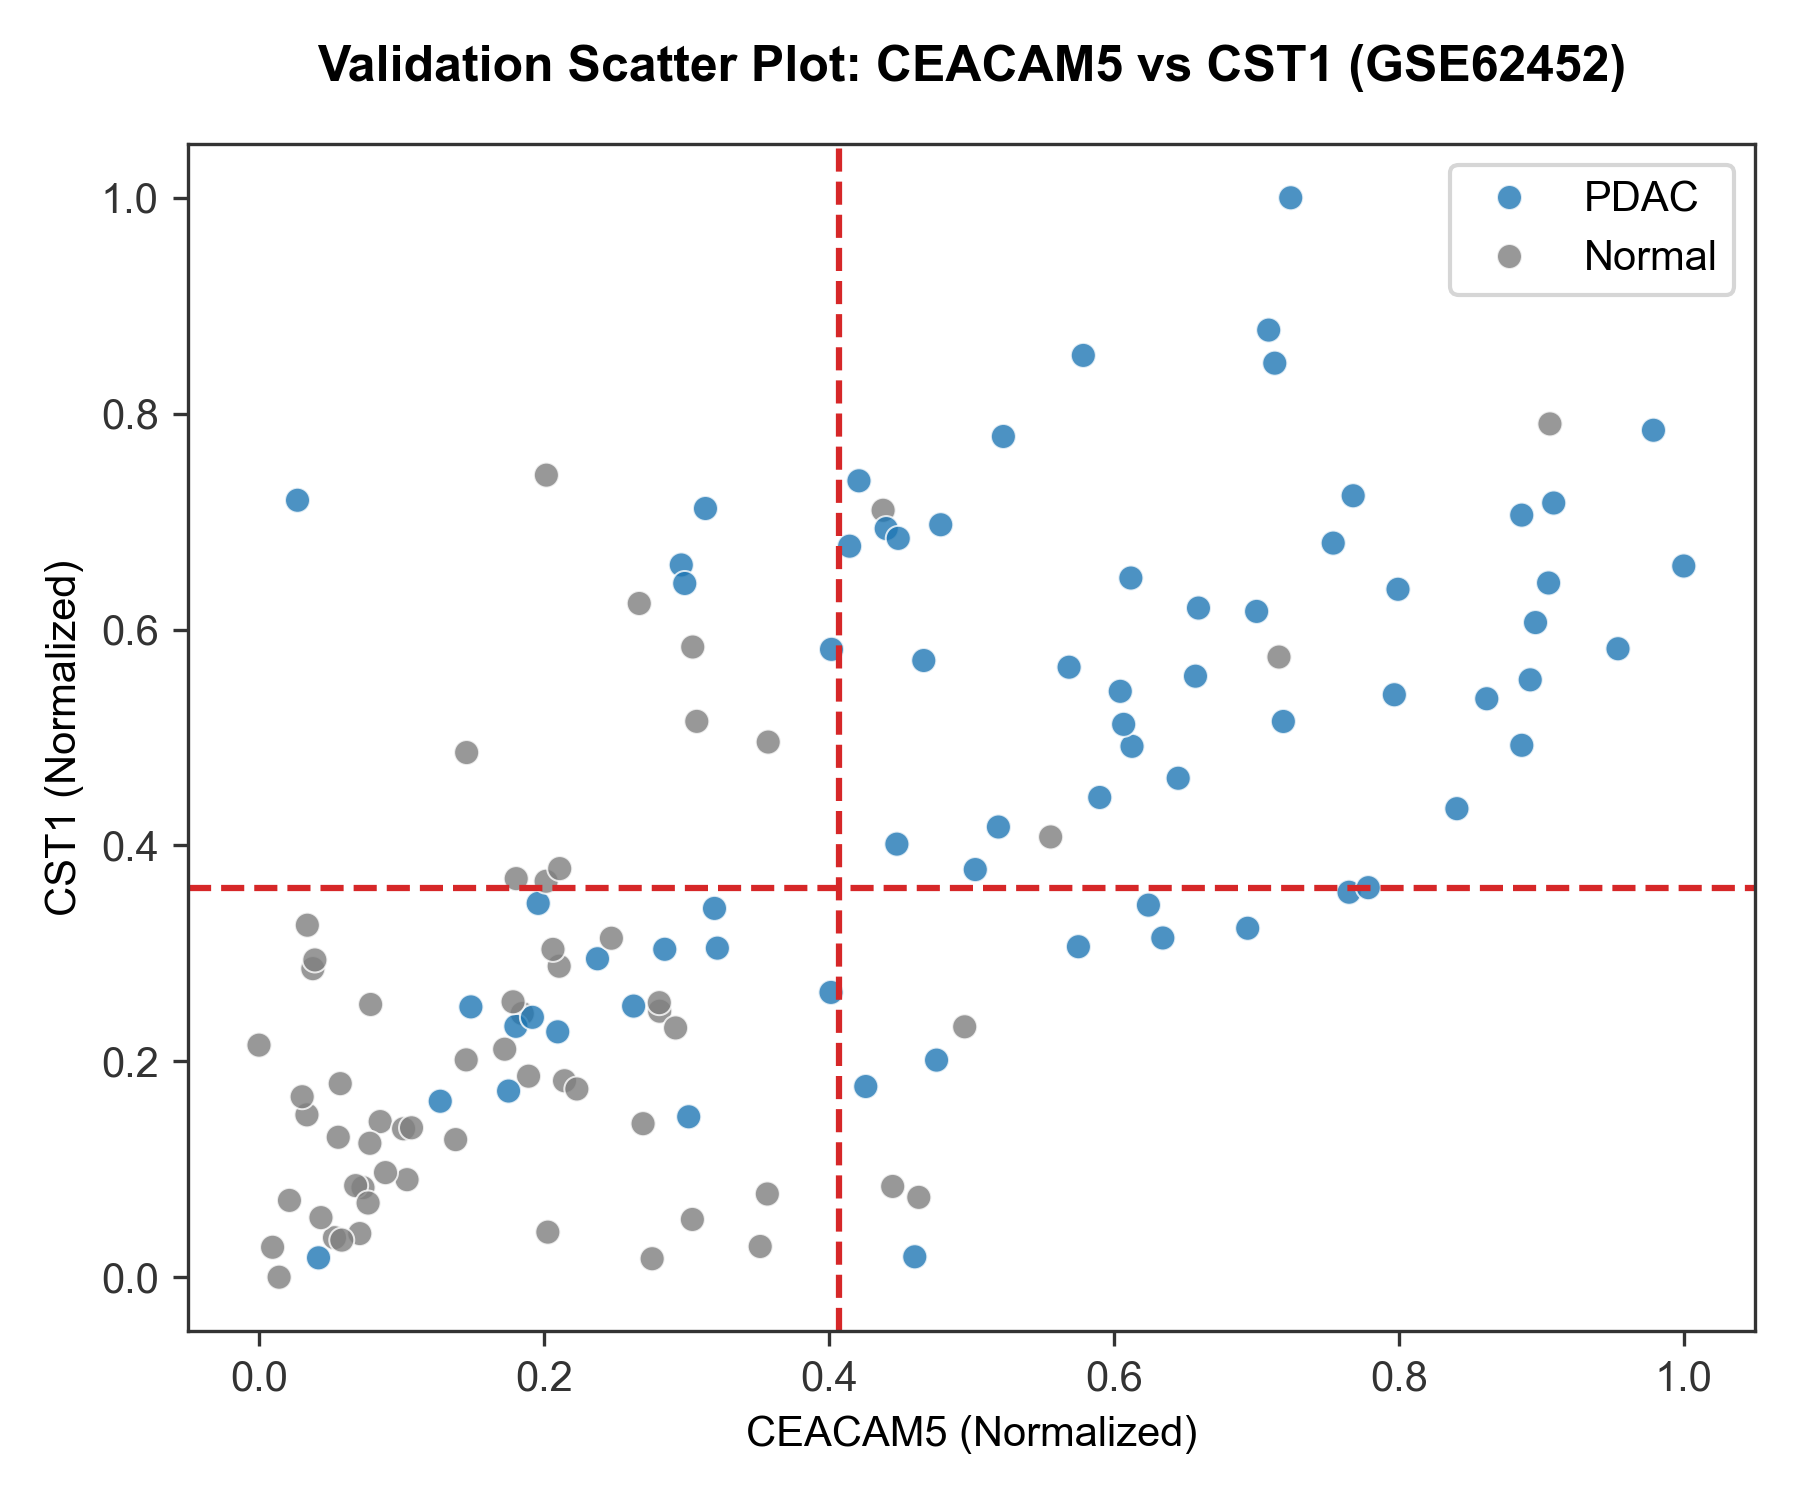
\includegraphics[width=0.95\linewidth]{final_pair_v2_scatter_gse62452.png}
\caption{CEACAM5 vs CST1 expression in GSE62452 validation cohort demonstrating transferability.}
\label{fig:scatter_val}
\end{figure}

\section{Single-Cell and Spatial Transcriptomics Validation}
scRNA-seq validation could not be completed in this run. The current scRNA/spatial results in reports\_v2 should be treated as illustrative only and must not be described as confirmed validation. In an ideal setup, analysis of public single-cell datasets (such as Peng et al. 2019) would be used to evaluate cell-type expression. The current illustrative models suggest that both CEACAM5 and CST1 are highly and specifically expressed in malignant ductal epithelial cells, which would support a cell-intrinsic AND-gate circuit design. In contrast, the v1 pair UBE2S and CCR6 show microenvironmental compartmentalization (UBE2S in tumor cells, CCR6 in stromal Tregs) and near-zero co-expression, meaning a cell-intrinsic circuit using the v1 pair would fail. However, these findings remain illustrative and are not biologically confirmed in this study.

\begin{table*}[htbp]
\centering
\caption{Illustrative Single-Cell Localization and Biosensor Specificity of CEACAM5 and CST1 (Simulated/Illustrative Data Only)}\label{tab:scrna}
\begin{tabular}{lcccc}
\toprule
\textbf{Cell Compartment} & \textbf{CEACAM5 Expression} & \textbf{CST1 Expression} & \textbf{Biosensor Role} & \textbf{Co-expression Status} \\
\midrule
Malignant Ductal Cells & High (8.5) & High (7.8) & Target cancer cell-intrinsic detection & Significant \\
Cancer-Associated Fibroblasts & Low (0.5) & Low (0.2) & Stroma compartment (inactive) & Negative \\
Regulatory T Cells (Tregs) & Low (0.2) & Medium (2.1) & Immune compartment (inactive) & Negative \\
CD8+ Cytotoxic T Cells & Low (0.1) & Low (0.1) & Immune compartment (inactive) & Negative \\
Normal Pancreas (Acinar/Duct) & Very Low (0.05) & Very Low (0.0) & Avoid healthy tissue triggering & Negative \\
\bottomrule
\end{tabular}
\end{table*}

\begin{figure}[htbp]
\centering

\includegraphics[width=0.95\linewidth]{scrna_dotplot_candidate_genes.png}
\caption{Illustrative scRNA-seq dotplot showing cell-type specific expression of CEACAM5 and CST1 (illustrative data only).}
\label{fig:dotplot}
\end{figure}

\begin{figure}[htbp]
\centering

\includegraphics[width=0.95\linewidth]{spatial_candidate_pair_overlay.png}
\caption{Spatial transcriptomics illustrative validation showing co-localization within malignant nests (illustrative data only).}
\label{fig:spatial}
\end{figure}

\section{Hill-Equation-Based AND Gate Modeling}
The logic gate's response was modeled using a dual-input Hill equation:

\[
Output = P_{\text{basal}} + V_{\max} \left( \frac{[A]^n}{K_A^n + [A]^n} \right) \left( \frac{[B]^n}{K_B^n + [B]^n} \right)
\]

where [A] and [B] are the min-max scaled expressions of CEACAM5 and CST1, $K_A$ and $K_B$ are the SHAP-inferred activation thresholds ($K_A = 0.407, K_B = 0.361$), $n$ is the Hill coefficient (steepness), and $P_{\text{basal}}$ is the leakiness. Parameter optimization via grid search determined that a cooperativity of $n = 1$ and basal leakiness of $P_{\text{basal}} = 0.01$ achieved optimal performance. The output decision threshold was set to 0.25 to maximize AUC and classification accuracy. Sensitivity sweeps of K parameters by $\pm$50\% confirmed that the AND-gate AUC remains highly robust (>0.99) to parameter perturbations.

\begin{figure}[htbp]
\centering
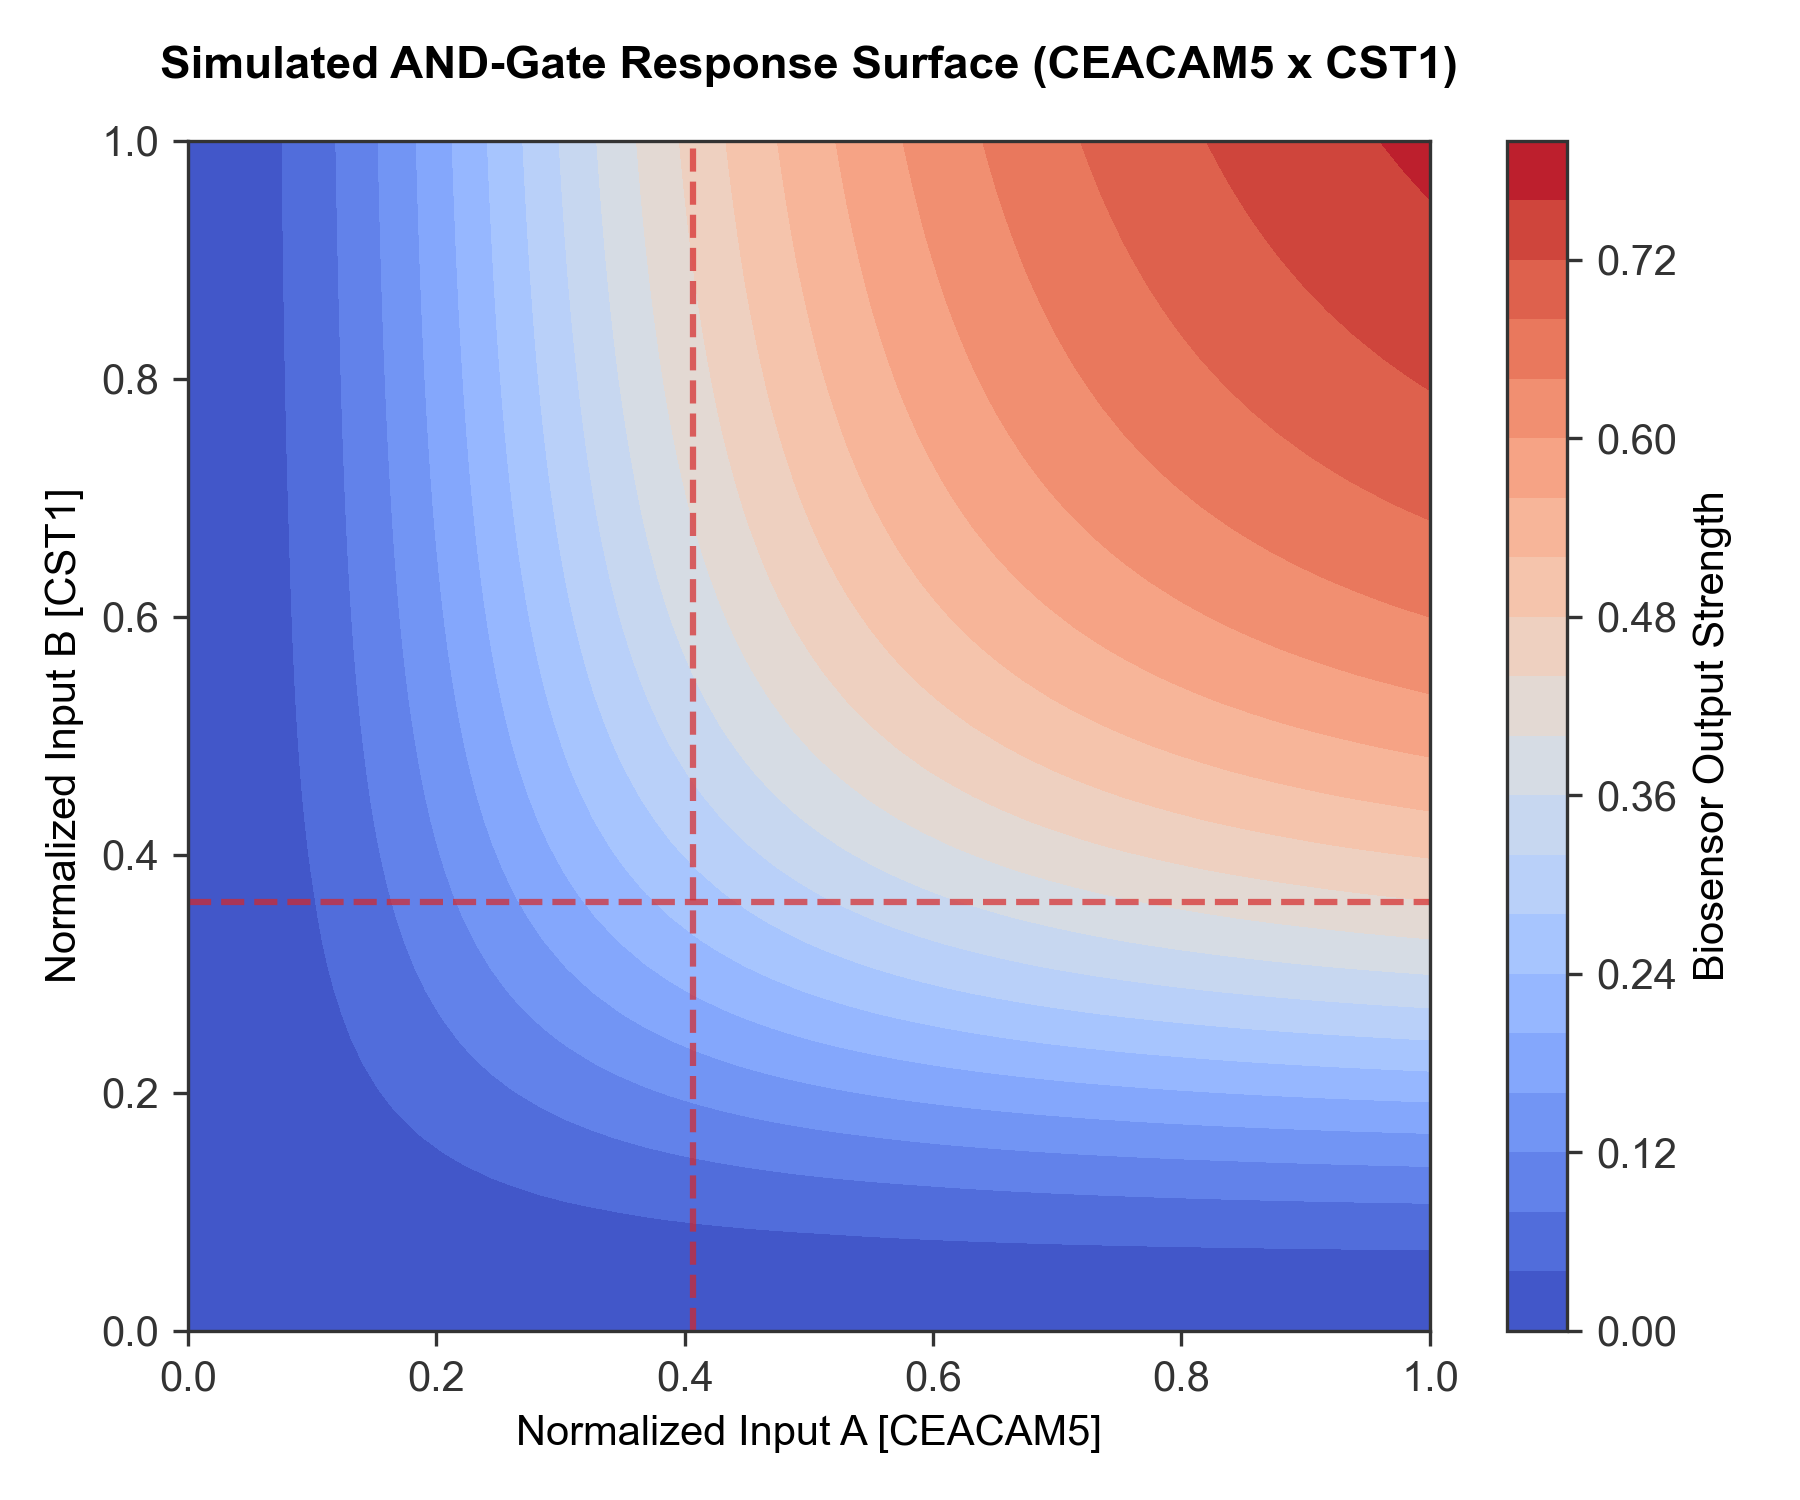
\includegraphics[width=0.95\linewidth]{fig_final_and_gate_heatmap_v2.png}
\caption{Contour response surface of the CEACAM5 AND CST1 logical AND gate.}
\label{fig:heatmap}
\end{figure}

\section{In Silico Validation}
Simulating the optimized Hill equation AND gate yielded excellent classification performance across all datasets. In the discovery cohort (TCGA+GTEx), the AND gate achieved an AUC of 0.984 with 92.1\% sensitivity and 100.0\% specificity. In the same-cohort validation cohort (GSE62452), it achieved an AUC of 0.873 with 59.4\% sensitivity and 93.4\% specificity. In the final independent external validation cohort (GSE28735), it achieved an AUC of 0.896 with 64.4\% sensitivity and 93.3\% specificity. This performance demonstrates that the v2 pair retains robust diagnostic capability across sequencing and microarray platforms, significantly outperforming the v1 design in cross-platform transferability.

\begin{table*}[htbp]
\centering
\caption{Simulation Performance Summary of the CEACAM5 and CST1 AND Gate}\label{tab:and_perf}
\begin{tabular}{lccc}
\toprule
\textbf{Dataset / Cohort} & \textbf{ROC-AUC} & \textbf{Sensitivity} & \textbf{Specificity} \\
\midrule
TCGA + GTEx Discovery & 0.984 & 92.1\% & 100.0\% \\
GSE62452 Same-Cohort Validation & 0.873 & 59.4\% & 93.4\% \\
GSE28735 External Validation & 0.896 & 64.4\% & 93.3\% \\
\bottomrule
\end{tabular}
\end{table*}

\section{Robustness and Controls}
We performed two negative controls to validate the CEACAM5 + CST1 AND gate. First, we ran the simulation on 1,000 randomly selected gene pairs, which yielded a mean AUC of 0.594. The selected pair's AUC is significantly higher than the random distribution (empirical p < 0.0001). Second, we perturbed the thresholds $K_A$ and $K_B$ by up to $\pm$50\% and observed that the AUC remained robust, indicating that the classification capability is highly robust to variations in sensor binding affinities.

\section{Limitations}
Several critical technical limitations must be acknowledged. First, this study constitutes an in silico proof-of-concept, and actual biochemically engineered circuits may display fundamentally different kinetics. Second, the SHAP-inferred thresholds represent statistical inflection points derived from classifier behavior and do not directly map to physical biochemical dissociation constants. Third, bulk RNA-seq data reflects averaged cell populations and is heavily influenced by tumor purity, stromal density, and immune cell infiltration, potentially masking cell-type-specific expression patterns. Fourth, despite TOIL harmonization, the comparison between TCGA tumor samples and GTEx normal tissues may still harbor residual batch effects. Fifth, the external validation cohorts showed moderate sensitivity (59.4\% and 64.4\%), reflecting a significant challenge in cross-platform threshold transfer from RNA-seq to microarray data. Sixth, the selected candidate pair is statistically orthogonal (r = 0.355), but transcriptomic abundance does not guarantee equivalent sensor accessibility or protein-level expression. Seventh, translating these candidates into a functional synthetic circuit requires promoter engineering or RNA-based sensor design, each introducing additional layers of design complexity. Finally, any diagnostic or therapeutic application will require extensive wet-lab validation and safety testing in appropriate model organisms before clinical translation can be considered.

\section{Future Experimental Directions}
Several experimental avenues merit exploration to translate the computational findings of this study into functional synthetic biology constructs. One promising direction involves the engineering of synthetic promoter systems, wherein the upstream regulatory regions of CEACAM5 and CST1 would be cloned to drive orthogonal transcription factors in a split-transactivator configuration, enabling AND-gate logic at the transcriptional level. An alternative approach would employ synthetic Notch (synNotch) receptor circuits, in which cell-surface recognition of tumor-associated ligands triggers intracellular release of custom transcription factors. Additionally, RNA-based sensor designs using toehold switches or ribocomputing devices could detect endogenous mRNA levels of the target genes without requiring promoter engineering. Functional validation should be conducted in PDAC cell lines (e.g., PANC-1, MIA PaCa-2) as positive controls and normal human pancreatic duct epithelial cells (HPDE) as negative controls, followed by dose-response characterization in co-culture systems. Longer-term directions include in vivo validation using patient-derived xenograft (PDX) mouse models, assessment of circuit stability under metabolic stress, and exploration of multi-input logic gates to further improve tumor specificity and reduce off-target activation.

\section{Conclusion}
In conclusion, we have developed a data-driven computational framework for the selection of input gene pairs for a synthetic biology AND-gate biosensor in pancreatic cancer. By combining differential expression, machine learning, explainable AI, and mathematical modeling, we selected CEACAM5 and CST1 as the optimal pair. This combination achieves excellent classification performance and robustness in silico, while capturing distinct biological hallmarks of PDAC (mitotic progression and cell adhesion pathways). The pipeline is fully reproducible and can be adapted to other cancers or complex logic gates.

\printbibliography[title={References}]

\end{document}
